\section{Ohmsches Gesetz}

Das Ohmsche Gesetz gehört zu den grundlegenden Prinzipien der Elektrotechnik. Es beschreibt den linearen Zusammenhang zwischen der Spannung $U$, der Stromstärke $I$ und dem Widerstand $R$ in einem elektrischen Stromkreis. Dieser Zusammenhang wird durch die Gleichung \eqref{eq:Ohm'sche Gleichung} beschrieben:
\begin{equation} \label{eq:Ohm'sche Gleichung}
    U = I \cdot R
\end{equation}
Zur Veranschaulichung des Ohmschen Gesetzes wird die in Abbildung \ref{fig:K2A1} dargestellte Schaltung aufgebaut. In diesem Experiment wird zunächst die Stromstärke $I$ in Abhängigkeit von der Spannung $U$ bei einem konstanten Widerstand $R$ gemessen und die Ergebnisse in Tabelle \ref{tab:K2T1} dokumentiert. Anschließend wird die Stromstärke $I$ in Abhängigkeit vom Widerstand $R$ bei einer konstanten Spannung $U$ erfasst und in Tabelle \ref{tab:K2T2} aufgeführt.

Die Messdaten werden jeweils grafisch aufbereitet, um den Zusammenhang in Form von Kennlinien darzustellen (siehe Abbildung \ref{fig:K2A2} und Abbildung \ref{fig:K2A3}). Diese grafische Auswertung dient der Überprüfung der Gültigkeit des Ohmschen Gesetzes.
\begin{figure}[H]
    \centering
    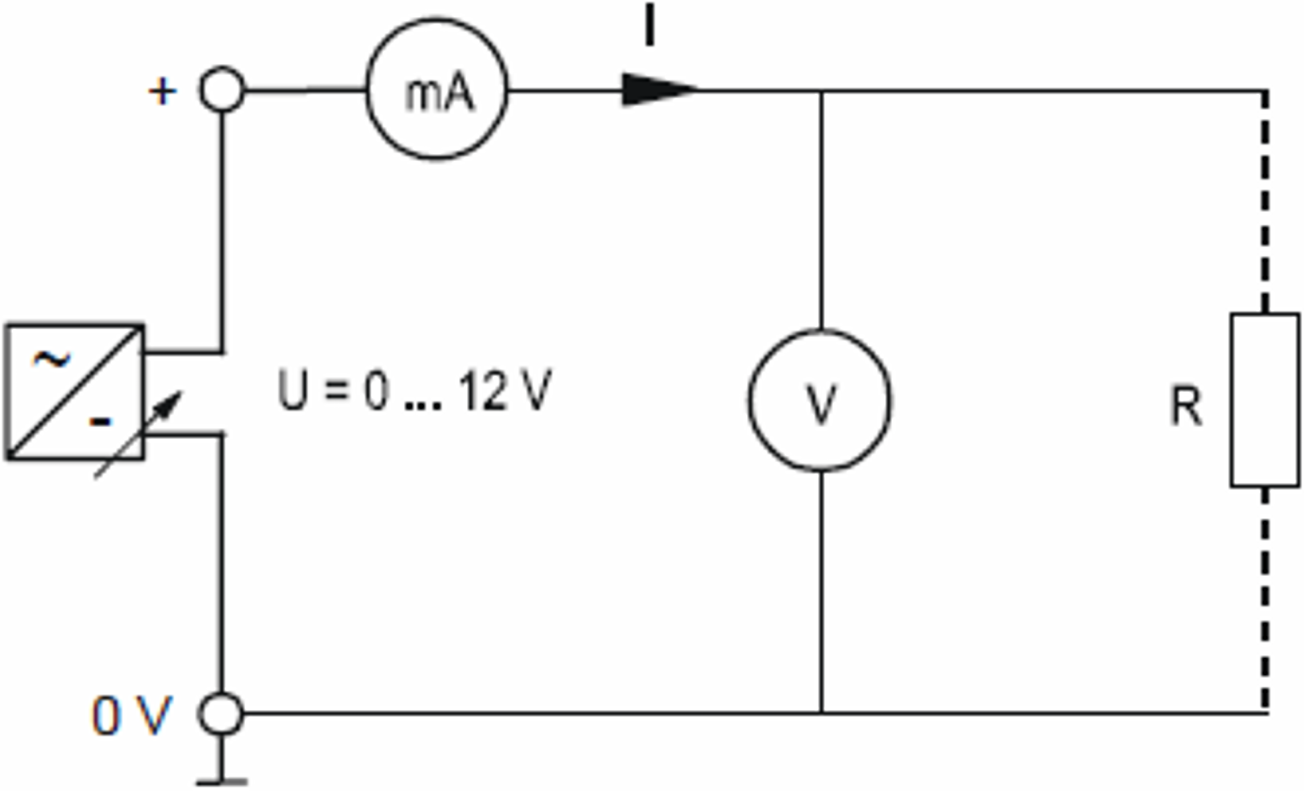
\includegraphics[width=0.5\textwidth]{Pictures/Kapitel2/Ohmsches Gesetz.png}
    \caption{Schematischer Aufbau des Stromkreises zur Untersuchung des Widerstands}
    \label{fig:K2A1}
\end{figure}

\subsection{Messwerte}
\begin{table}[H]
\centering
\caption{Gemessene Werte für $I$ in Abhängigkeit von $U$ bei konstantem $R$}
\begin{tabular}{ c c c c c c c c } % Abstand der Spalten
\toprule
    $U/\,\unit{V}$& 0 & 2 & 4 & 6 & 8 & 10 & 12\\
     \midrule
    $I/\,\unit{mA}$ bei $100\,\unit{\Omega}$&0,0 & 19,8 & 39,6 & 59,2 & 78,8 & 98,4 & 117,6\\
    $I/\,\unit{mA}$ bei $300\,\unit{\Omega}$& 0,0 & 6,1 & 12,2 & 18,3 & 24,5 & 30,7 & 36,8\\
    \bottomrule
\end{tabular}{}
\label{tab:K2T1}%Kapitel1 Ohmsches Gesetz Tabelle1
\end{table}{}

\begin{table}[H]
\centering
\caption{Gemessene Werte für $I$ in Abhängigkeit von $R$ bei konstanter $U$}
\begin{tabular}{ c c c c c c c } % Abstand der Spalten
\toprule
    $R/\,\unit{\Omega}$& 100 & 220 & 330 & 470 & 680 & 1000\\
     \midrule
    $I/\,\unit{mA}$ bei $\SI{12}{\V}$&118,20 & 54,30 & 36,87 & 25,64 & 17,76 & 12,24\\
    $I/\,\unit{mA}$ bei $\SI{8}{\V}$& 79,00 & 36,33 & 24,55 & 17,05 & 11,81 & 8,13\\
    $I/\,\unit{mA}$ bei $\SI{4}{\V}$& 39,60 & 18,19 & 12,29 & 8,53 & 5,90 & 4,06\\
    \bottomrule
\end{tabular}{}
\label{tab:K2T2}%Kapitel1 Ohmsches Gesetz Tabelle2
\end{table}{}

\vspace{0.5cm}

\begin{figure}[H]
\centering
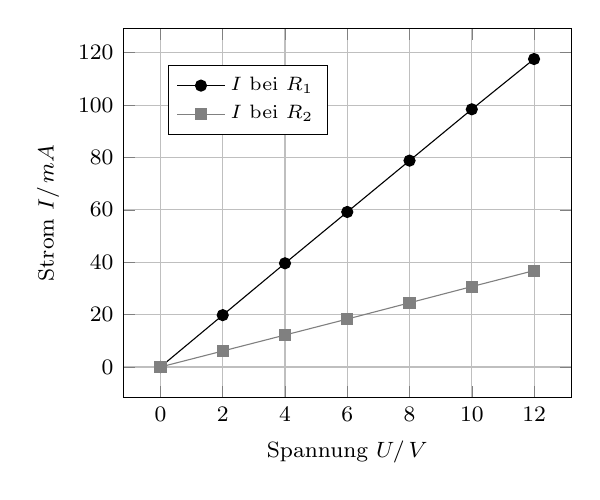
\begin{tikzpicture}
\begin{axis}[
    width=0.6\textwidth,
    xlabel={Spannung $U/\,\unit{V}$},
    ylabel={Strom $I/\,\unit{mA}$},
    grid=major,
    legend style={at={(0.1,0.9)}, anchor=north west, font=\scriptsize},
    xtick={0,2,4,6,8,10,12},
    ytick={0,20,40,60,80,100,120},
    font=\footnotesize
]
% R1 Daten
\addplot[mark=*,black] coordinates {(0, 0) (2, 19.8) (4, 39.6) (6, 59.2) (8, 78.8) (10, 98.4) (12, 117.6)};
\addlegendentry{$I$ bei $R_1$}

% R2 Daten
\addplot[mark=square*,gray] coordinates {(0, 0) (2, 6.1) (4, 12.2) (6, 18.3) (8, 24.5) (10, 30.7) (12, 36.8)};
\addlegendentry{$I$ bei $R_2$}

\end{axis}
\end{tikzpicture}
\caption{Kennlinie $I = f(U)$ bei konstantem Widerstand}
\label{fig:K2A2}
\end{figure}

\begin{figure}[H]
\centering
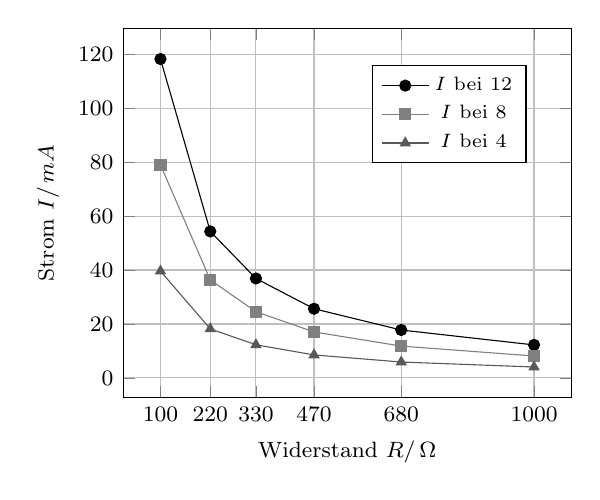
\begin{tikzpicture}
\begin{axis}[
    width=0.6\textwidth,
    xlabel={Widerstand $R/\,\unit{\Omega}$},
    ylabel={Strom $I/\,\unit{mA}$},
    grid=major,
    legend style={at={(0.9,0.9)}, anchor=north east, font=\scriptsize},
    xtick={100,220,330,470,680,1000},
    xticklabels={100,220,330,470,680,1000},
    ytick={0,20,40,60,80,100,120},
    font=\footnotesize,
    %xmode=log,
    %log basis x={10}
]

% U = 12V Daten
\addplot[mark=*,black] coordinates {(100, 118.20) (220, 54.30) (330, 36.87) (470, 25.64) (680, 17.76) (1000, 12.24)};
\addlegendentry{$I$ bei $\SI{12}{\V}$}

% U = 8V Daten
\addplot[mark=square*,gray] coordinates {(100, 79.00) (220, 36.33) (330, 24.55) (470, 17.05) (680, 11.81) (1000, 8.13)};
\addlegendentry{$I$ bei $\SI{8}{\V}$}

% U = 4V Daten
\addplot[mark=triangle*,gray!70!black] coordinates {(100, 39.60) (220, 18.19) (330, 12.29) (470, 8.53) (680, 5.90) (1000, 4.06)};
\addlegendentry{$I$ bei $\SI{4}{\V}$}

\end{axis}
\end{tikzpicture}
\caption{Kennlinie $I = f(R)$ bei konstanter Spannung}
\label{fig:K2A3}
\end{figure}

\subsection{Rechnerische Überprüfung}

Zur Überprüfung der gemessenen Werte (siehe Tabelle \ref{tab:K2T3} und \ref{tab:K2T4}) wird das Ohmsche Gesetz herangezogen, siehe Anhang \ref{appA}.

\begin{table}[H]
\centering
\caption{Rechnerisch ermittelte Werte für $I$ bei konstantem $R$}
\begin{tabular}{ c c c c c c c c } % Abstand der Spalten
\toprule
    $U/\,\unit{V}$& 0 & 2 & 4 & 6 & 8 & 10 & 12\\
     \midrule
    $I/\,\unit{mA}$ bei $100\,\unit{\Omega}$ & 
    0,0 & 20,0 & 40,0 & 60,0 & 80,0 & 100,0 & 120,0\\
    $I/\,\unit{mA}$ bei $300\,\unit{\Omega}$ & 
    0,0 & 6,7 & 13,3 & 20,0 & 26,7 & 33,3 & 40,0\\
    \bottomrule
\end{tabular}
\label{tab:K2T3}%Rechnerische Tabelle1
\end{table}

\begin{table}[H]
\centering
\caption{Rechnerisch ermittelte Werte für $I$ bei konstantem $U$}
\begin{tabular}{ c c c c c c c } % Abstand der Spalten
\toprule
    $R/\,\unit{\Omega}$ & 100 & 220 & 330 & 470 & 680 & 1000\\
     \midrule
    $I/\,\unit{mA}$ bei $\SI{12}{\V}$ & 120,0 & 54,6 & 36,4 & 25,5 & 17,7 & 12,0\\
    $I/\,\unit{mA}$ bei $\SI{8}{\V}$ & 80,0 & 36,4 & 24,2 & 17,0 & 11,8 & 8,0\\
    $I/\,\unit{mA}$ bei $\SI{4}{\V}$ & 40,0 & 18,2 & 12,1 & 8,5 & 5,9 & 4,0\\
    \bottomrule
\end{tabular}
\label{tab:K2T4}%Rechnerische Tabelle2
\end{table}

Die Abweichungen zwischen den gemessenen und den berechneten Werten sind minimal und können auf Messungenauigkeiten oder Rundungsfehler zurückzuführen sein. Insgesamt stimmen die Werte gut mit dem Ohmschen Gesetz überein.

\newpage
